%%% Fiktivní kapitola s instrukcemi k PDF/A

\chapter{Kreslení} \label{kresleni}

Přirozenou snahou pro studování nalezených grafů, a pochopení, proč některé nelze najít, je hledat jejich zobrazení, které je pro člověka dostatečně čitelné. Překvapivě, i přes rovinnost grafů a celkem dobré znalosti jejich struktury není jednoduché hezké rovinné nakreslení najít.

Zamysleme se, jak graf bude vypadat. Vrcholy, které mají ležet na vnější stěně, rozmístěme po~kružnici a pak - podle jednotlivých hranic, které graf řeší - vždy vrcholy nově uzavřené stěny nakresleme na~soustřednou, menší kružnici tak, aby spojnice žádného bodu hranice se středem kružnic neprotínala jiný bod hranice. Tímto způsobem určitě získáme rovinné nakreslení (ale hrany mohou být libovolné křivky), protože v~každém kroku je možné spojit libovolné dva vrcholy, které mohou být v řešení zrovna spojovány, tak, abychom zachovali požadovanou vlastnost tvaru hranice.

Problémem takového nakreslení je počet soustředných kružnic, které bychom potřebovali, který odpovídá počtu stěn grafu. Množství potřebných kružnic by šlo celkem jednoduše snížit. Nově přidávané vrcholy nakreslíme vždy na největší kružnici, na které v příslušné výseči ještě žádný vrchol neleží. Dalším problémem by bylo rozložení vrcholů do výsečí. Představme si třeba zadání, ve kterém značný podíl tvoří souvislá posloupnost \uv{out} vrcholů. Pokud ve výpočtu dojde k uzavření stěny, která tyto vrcholy obsahuje, až na závěr, bude výseč, ve které leží, jinak zcela prázdná.

Další možností jsou běžně dostupné programy či funkce na kreslení grafů. Posouzení jejich kvality na náhodném z malých nalezených grafů necháváme na~čtenáři.


\begin{figure}[h]\centering
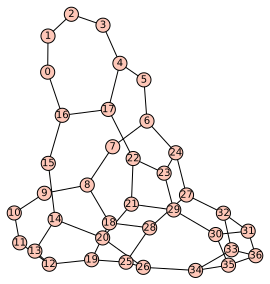
\includegraphics[width = 60mm]{../img/sageplot}
\caption{Automatické nakreslení SageMath \cite{sagemath}. Všimněme si, pokud bychom si zkusili představit, že cyklus vrcholů 0, 1, $\dots$, 16 je ona vnější kružnice z vylepšeného prvního popsaného kreslení a navíc nechť je základnou kužele a všechny další kružnice nechť jsou vždy v tomto kuželu výš (tak, aby mohly ležet na plášti), pak (s množstvím fantazie) se koukáme na podobné nakreslení, jen popsané je pohled shora a zobrazené pohled z boku. Při nakreslení většího grafu je tato myšlenka viditelnější.}
\label{obr:sageplot}
\end{figure}


\begin{figure}[h]\centering
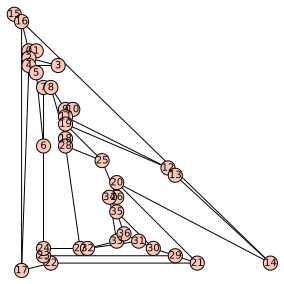
\includegraphics[width = 60mm]{../img/planar}
\caption{Rovinné nakreslení SageMath.}
\label{obr:planar}
\end{figure}


\begin{figure}[h]\centering
\includegraphics[width = 60mm]{../img/Triarc15150{4,7}__v37}
\caption{Neato s předdefinovanými pozicemi vnější stěny.}
\label{obr:Triarc15150{4,7}__v37}
\end{figure}



Nejuspokojivější nalezenou možností je Tuttův (barycentrický) algoritmus. Jak název napovídá, jde o umisťování vrcholů do \uv{těžišť}. Nejprve je třeba rozdělit vrcholy do dvou skupin: pevné a volné. Pevné vrcholy jsou rozestaveny, aby tvořily konvexní n-úhelník. Pozice volných vrcholů se pak dopočítá jako vážený průměr sousedních vrcholů, tedy stačí řešit soustavu lineárních rovnic.

Aby mohl algoritmus dobře fungovat, je nutné, aby graf byl 3-souvislý (že jde i o postačující podmínku ukazuje článek  \cite{Tutte}). Pokud by nebyl 3-souvislý, pak vrcholy komponenty, která by po odebrání dvou vrcholů byla oddělena od zbytku grafu a neobsahovala by pevné vrcholy, budou ležet v jedné přímce.

\begin{tvrz} \label{prevodNa3Spoj}
Mějme graf $G=(V,E)$ a seznam jeho stěn $F$, oboje získané algoritmem z Kapitoly \ref{resitko}. Pro každou stěnu $f \in F$ vytvořme nový vrchol $v_f$ a buď $V^*$ množina těchto vrcholů.  Pak graf $G^* = (V \cup V^*, E \cup \lbrace \lbrace u,v \rbrace \mid u_f \in V^*, v \in f, f \in F\rbrace$ je 3-souvislý.
\end{tvrz}

\begin{dukaz}
Pro spor nechť jsou vrcholy $u,v  \in V\cup V^*$ takové, že po~jejich odebrání se graf $G^*$ rozpadne na více komponent. Ze způsobu, kterým graf vzniká, víme, že je 2-souvislý, a proto ani jeden z $u,v$ není z $V^*$. Označme vrcholy $a,b$, mezi kterými po odebrání $u,v$ nevede cesta, nechť $P$ je cesta, která je spojuje v~$G^*$ a~bez~újmy na~obecnosti díky 2-souvislosti nechť $u \in P$ a $v \notin P$. Pak vrcholy těsně před a~po~$u$ v~$P$ sdílí v~$G$ nějakou stěnu $f$ (protože v $G$ mají vrcholy stupeň nejvýše 3) a tedy lze P upravit vyměněním $u$ za $v_f$, která spojuje $a$ a $b$ v grafu po odebrání $u,v$, což je spor s volbou $a$ a $b$.
\end{dukaz}

Pro převedení grafu na 3-souvislý stačí tedy do každé stěny vložit nový vrchol a spojit ho se všemi vrcholy dané stěny. Pak zbývá zvolit pevné vrcholy -- v našem případě volíme vrcholy původní vnější stěny, které rozmístíme na kružnici a podle konkrétního grafu je pak možné nastavit váhy jednotlivých vrcholů. Obecně se pro dostatečně malé grafy (do 40-ti vrcholů) osvědčila lineární závislost váhy na~pořadí přidání vrcholu do grafu, nejdříve přidaný je nejtěžší. Skript, ve kterém lze Tuttovo nakreslení spočítat je jedním z výstupních formátů přiložené aplikace, více v Sekci \ref{prg&vystupy}.


\begin{figure}[h]\centering
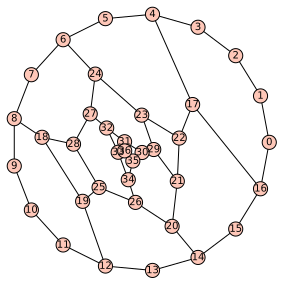
\includegraphics[width = 60mm]{../img/tutteplot}
\caption{Tuttovo nakreslení.}
\label{obr:tutteplot}
\end{figure}